
\chapter{Exercise 4}
\label{cha:ugeopgave-4}

The purpose of this exercise is to get acquainted with lighting and shading in OpenGL and GLSL.

\section{Part 1}
\label{sec:del-1:-newpaint}

I succeed with the part by following the suggested order given. The key point of this part is to consider that the \emph{lightPosition} in the shader is in eye-coordinates.\\
The result can be seen in Figure \ref{fig:4-1}.




\begin{figure}[hp]
\centering
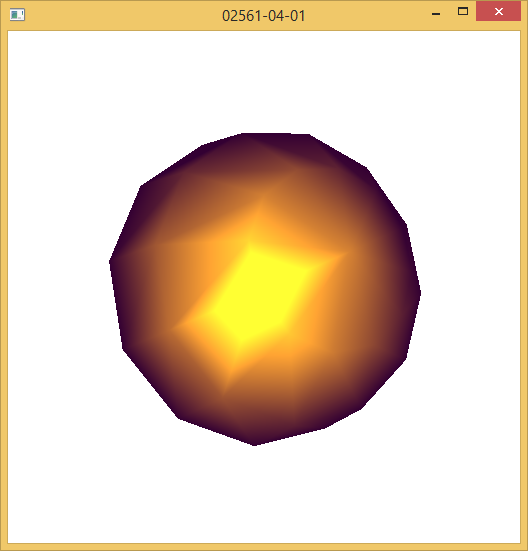
\includegraphics[width=8cm]{../Screenshots/ex-4/1.png}
\caption{Gouraud Shading}
\label{fig:4-1}
\end{figure}










\section{Part 2}
\label{sec:del-2:-select-pick-picks}


I succeed with the part by following the suggested order given. User can toggle between directional and point light model by pressing \emph{L} key on keyboard.
The result with directional light can be seen in Figure \ref{fig:4-2-1}. On the other hand, the result with point light source can be seen in Figure \ref{fig:4-2-2}.\\
\emph{Shininess is set to 20 in this part.}



\begin{figure}[hp]
\centering
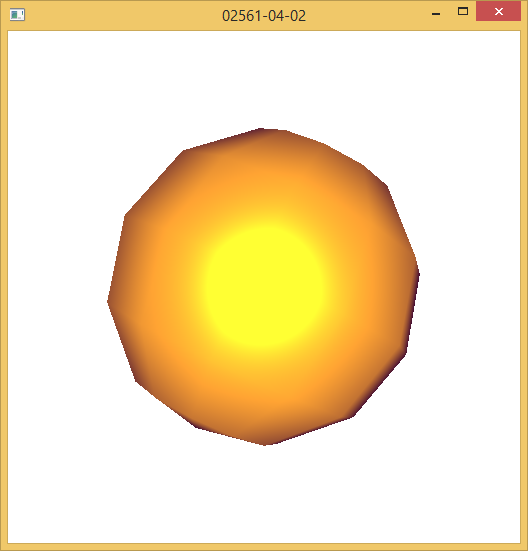
\includegraphics[width=8cm]{../Screenshots/ex-4/2-1.png}
\caption{Directional Light Source}
\label{fig:4-2-1}
\end{figure}

\begin{figure}[hp]
\centering
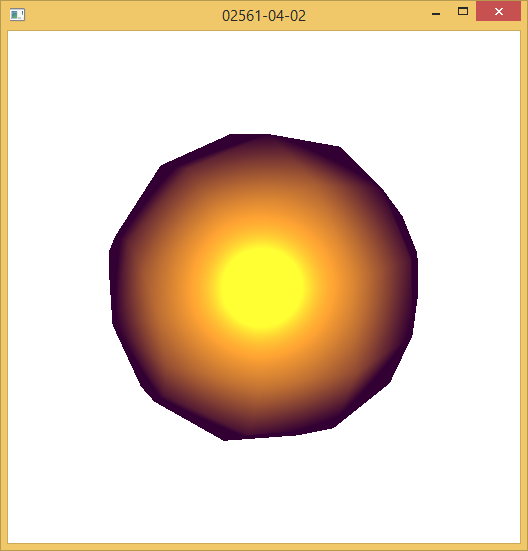
\includegraphics[width=8cm]{../Screenshots/ex-4/2-2.png}
\caption{Point Light Source}
\label{fig:4-2-2}
\end{figure}





\section{Part 3}
\label{sec:line-singledouble-logik}
\begin{itemize}
  \item Phong shading is a appliation of phong lightning. If you consider each pixels' normal during phong lightning calculation, it is phong shading.

  \item If you assign each polygon defined by vertices a normal, it is Gouraud's method. Calculations are done before rasterizing.
If you assign each pixel a normal, it is Phong's method. Calculations are done after rasterizing (fragment shading).
Gouraud's method is deceptively simple and Easy to compute as against Phong shading.
  \item Unlike point light, rays are parallel to each other in directional light.

  \item Yes. to make an analogy, the more rays your eyes reached to, the brighter you see where you look at.
  \item Surfaces looks dull without it, somewhat like chalk. What we are missing are the highlights that we see re?ected from shiny objects.
  \item As shininess is increased, the re?ected light is concentrated in a narrower region centered on the angle of a perfect re?ector.
  \item Instead of computing reflection for every point on surface, we have replaced r*v component with n*h, where r is reflection and
h is halfway vector. It is a succesful and efficient technique when used on flat or curved surfaces.
  \item In some cases, i.e. when modelView matrix makes non-uniform transformations, modelView matrix cannot be used to convert normal vectors
in object space to eye space coordinates. In such cases, normal matrix is used. It is equal to $ (M^{-1})^T $ where is upper left
3x3 matrix of modelView matrix.
 \item Eye space. Otherwise eye position dependent effects, such as specular lights would be harder to implement.

\end{itemize}

\section{Part 4}
\label{sec:diagramprogram}

I implement and complete part 5. Therefore I complete the objectives in Part 4. 
I add three light sources in positions $( 0.0, 0.0, -1.0)$, $( -3.0, -3.0, -1.0)$, and $(3.0, 3.0, -1.0)$. \\

The reader should follow the Part 5 to learn more about multiple light sources.

\section{Part 5}
\label{del-5}

Material color (ambient, diffuse and specular) is changed into a fragment shader uniform. Light color (ambient, diffuse and specular) is changed into a fragment shader uniform. One diffuse and specular color is assigned to each light position. Ambient-product, diffuse-product and specular-product is computed in the fragment shader and removed as a shader-uniform. I set the light diffuse color to be red, green and blue.\\
\emph{I set the shininess value to 100.} \\
You can see resulting screenshot in Figure \ref{fig:4-5}.


\begin{figure}[hp]
\centering
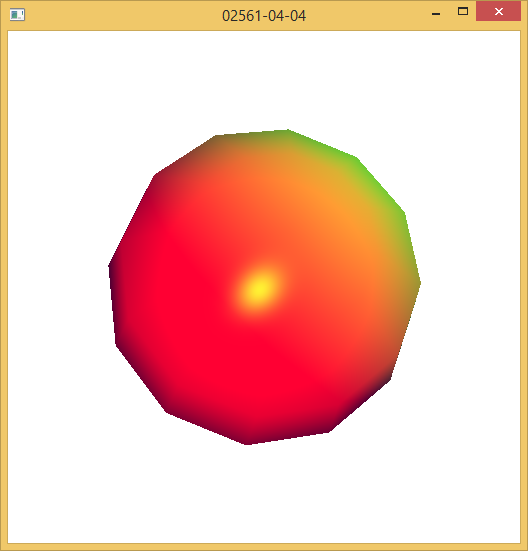
\includegraphics[width=8cm]{../Screenshots/ex-4/4.png}
\caption{Three point light source with different colors}
\label{fig:4-5}
\end{figure}
